\everymath{\displaystyle}
\documentclass{beamer}
% \documentclass[handout]{beamer}

%\usepackage[pdftex]{color,graphicx}
\usepackage{amsmath,amssymb,amsfonts}

\mode<presentation>
{
  % \usetheme{Darmstadt}
  % \usetheme[hideothersubsections]{Hannover}
  % \usetheme[hideothersubsections]{Goettingen}
  \usetheme[hideothersubsections, right]{Berkeley}

  \usecolortheme{seahorse}
  % \usecolortheme{dolphin}
  \usecolortheme{rose}
  % \usecolortheme{orchid}

  \useinnertheme[shadow]{rounded}

  % \setbeamercovered{transparent}
  \setbeamercovered{invisible}
  % or whatever (possibly just delete it)
}

\mode<handout>{
  \setbeamercolor{background canvas}{bg=black!5}
  \usepackage{pgfpages}
  \pgfpagesuselayout{4 on 1}[a4paper,border shrink=5mm, landscape]
}

\usepackage[brazilian]{babel}
% or whatever

% \usepackage[latin1]{inputenc}
\usepackage[utf8]{inputenc}
% or whatever

\usepackage{times}
%\usepackage[T1]{fontenc}
% Or whatever. Note that the encoding and the font should match. If T1
% does not look nice, try deleting the line with the fontenc.

\usepackage{ulem}

\title%[] % (optional, use only with long paper titles)
{Regressão Linear Simples}

\subtitle
{Modelos Estatísticos Aplicados} % (optional)

\author%[] % (optional, use only with lots of authors)
{Felipe Figueiredo}% \and S.~Another\inst{2}}
% - Use the \inst{?} command only if the authors have different
%   affiliation.

\institute[INTO] % (optional, but mostly needed)
{Instituto Nacional de Traumatologia e Ortopedia
}
  % \inst{1}%
  % Department of Computer Science\\
  % University of Somewhere
  % \and
  % \inst{2}%
  % Department of Theoretical Philosophy\\
  % University of Elsewhere}
% - Use the \inst command only if there are several affiliations.
% - Keep it simple, no one is interested in your street address.

\date%[] % (optional)
{}

% \subject{Talks}
% This is only inserted into the PDF information catalog. Can be left
% out. 



% If you have a file called "university-logo-filename.xxx", where xxx
% is a graphic format that can be processed by latex or pdflatex,
% resp., then you can add a logo as follows:

\pgfdeclareimage[height=1.6cm]{university-logo}{../logo}
\logo{\pgfuseimage{university-logo}}



% Delete this, if you do not want the table of contents to pop up at
% the beginning of each subsection:
\AtBeginSubsection[]
%\AtBeginSection[]
{
  \begin{frame}<beamer>{Sumário}
    \tableofcontents[currentsection,currentsubsection]
  \end{frame}
}


% If you wish to uncover everything in a step-wise fashion, uncomment
% the following command: 

% \beamerdefaultoverlayspecification{<+->}


\begin{document}

\begin{frame}
  \titlepage
\end{frame}

\begin{frame}{Sumário}
  \tableofcontents
  % You might wish to add the option [pausesections]
\end{frame}


%% Template
% \section{}

% \subsection{}

% \begin{frame}{}
%   \begin{itemize}
%   \item 
%   \end{itemize}
% \end{frame}

% \begin{frame}
%   \begin{columns}
%     \begin{column}{5cm}
%     \end{column}
%     \begin{column}{5cm}
%     \end{column}
%   \end{columns}
% \end{frame}

% \begin{frame}{}
%   \includegraphics[height=0.4\textheight]{file1}
%   \includegraphics[height=0.4\textheight]{file2}
%   \includegraphics[height=0.4\textheight]{file3}
%   \begin{figure}
%     \caption{}
%   \end{figure}
% \end{frame}

% \begin{frame}{}
%   \begin{definition}
%   \end{definition}
%   \begin{example}
%   \end{example}
%   \begin{block}{Exercício}
%   \end{block}
% \end{frame}

\section{Modelagem}

\subsection{Modelos em geral}

\begin{frame}{Modelos}
  \centering
  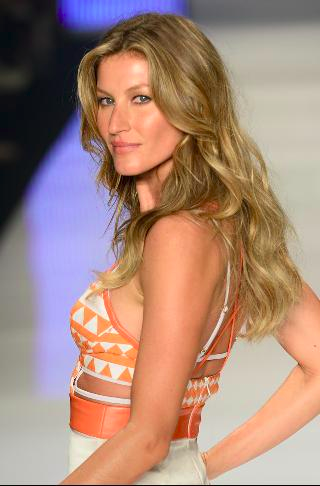
\includegraphics[height=\textheight]{Cap18-19/gi}
\end{frame}

\begin{frame}{Modelos animais}
  \centering
  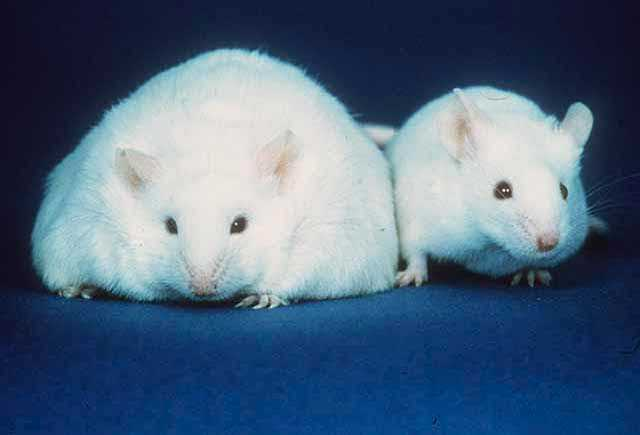
\includegraphics[width=\textwidth]{Cap18-19/Fatmouse}
\end{frame}

\begin{frame}{Modelos animais}
  \centering
  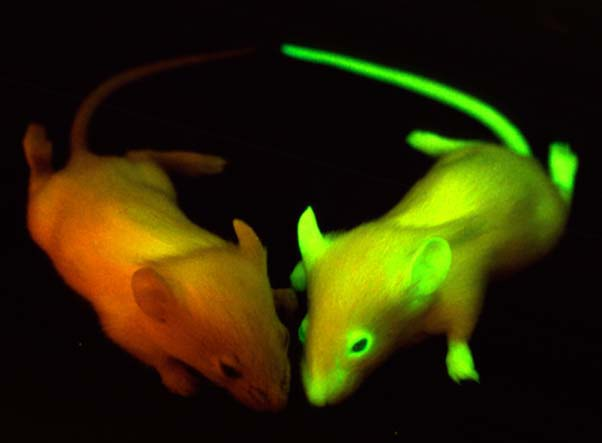
\includegraphics[width=\textwidth]{Cap18-19/GFP_hiir}
\end{frame}

\subsection{Modelos estatísticos}

\begin{frame}{Modelos estatísticos}
  Modelos servem para:
  \begin{itemize}
  \item representar de forma simplificada fenômenos, experimentos,
    dados, etc;
  \item possibilitar análise em cenários controlados, menos complexos
    que a realidade;
  \item extrapolar resultados e conclusões.
  \end{itemize}
\end{frame}

\begin{frame}{Modelos estatísticos}
  Ao ajustar um modelo aos dados, podemos:
  \begin{itemize}
  \item fazer predições dentro do intervalo observado para dados que
    não foram obtidos (interpolação)
  \item fazer predições fora do intervalo observado (extrapolação)
  \end{itemize}
\end{frame}

\begin{frame}{Para todos os gostos...}
  \begin{center}
    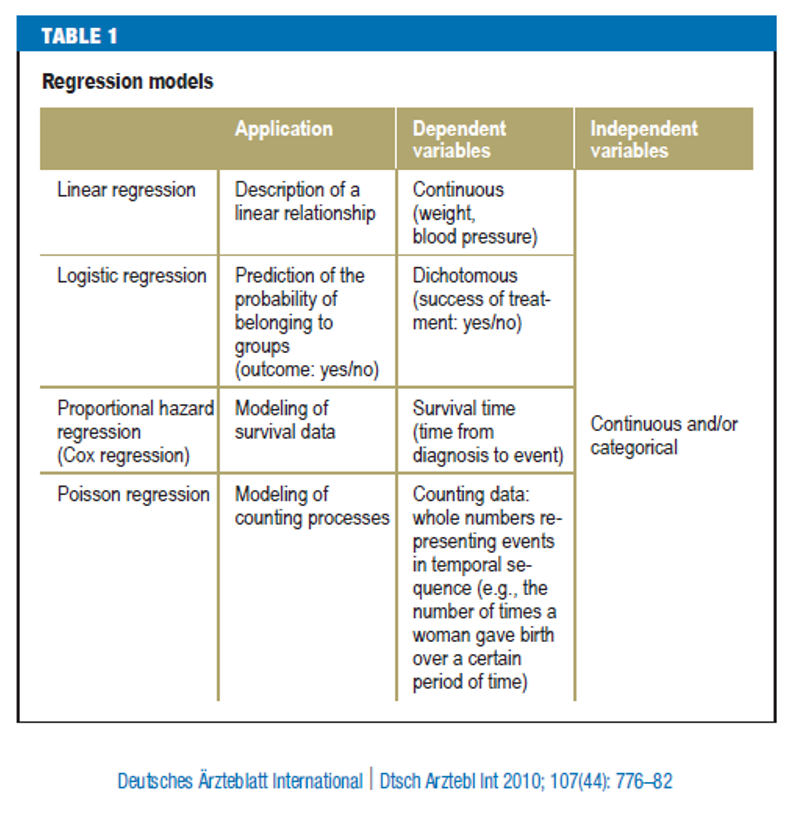
\includegraphics[height=.9\textheight]{Cap18-19/modelos-table1}
  \end{center}
\end{frame}

\section[Regressão]{Regressão Linear Simples}

\subsection{Introdução}

\begin{frame}{Modelo de regressão linear simples}
  \begin{block}{}
      Quando os dados indicam uma relação linear, um modelo de regressão pode ser utilizado para quantificar esta relação com uma {\bf reta de regressão}.
    \end{block}
  \begin{exampleblock}{Exemplo: Algumas aplicações}
%    Exemplos de perguntas que podem ser respondidas por tal modelo:

    \begin{itemize}
    \item Tendência (``Níveis de insulina em jejum tendem a aumentar com a idade?'')
    \item Ajuste de curva (``Qual é o EC$_{50}$ de uma nova droga?'')
    \item Predição (``Como predizer o risco de infarto do miocárdio, sabendo-se a idade, pressão e nível de colesterol?'')
    \end{itemize}
  \end{exampleblock}
\end{frame}

\begin{frame}{Depois dos comerciais...}
  \begin{center}
    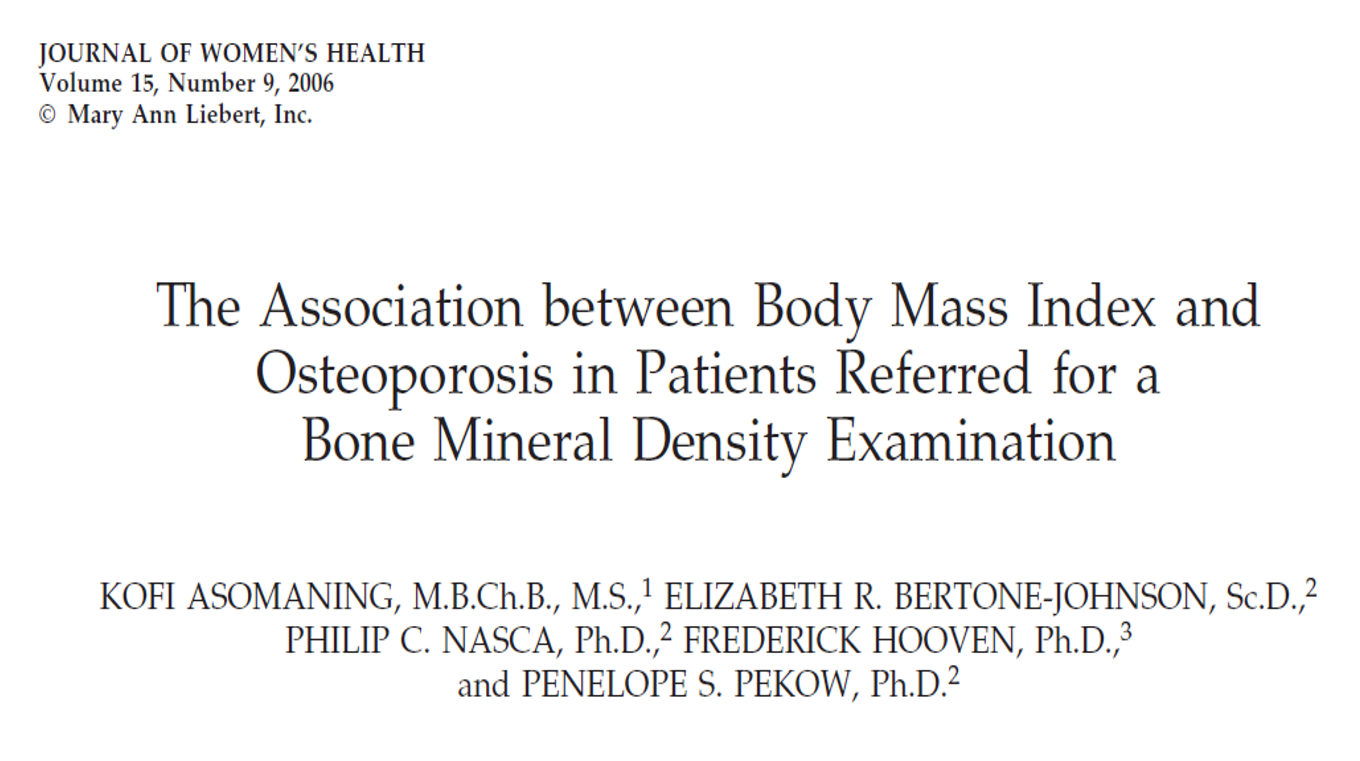
\includegraphics[width=\textwidth]{Cap18-19/bmi-bmd-title}
  \end{center}
\end{frame}

\begin{frame}{Depois dos comerciais...}
  \begin{center}
    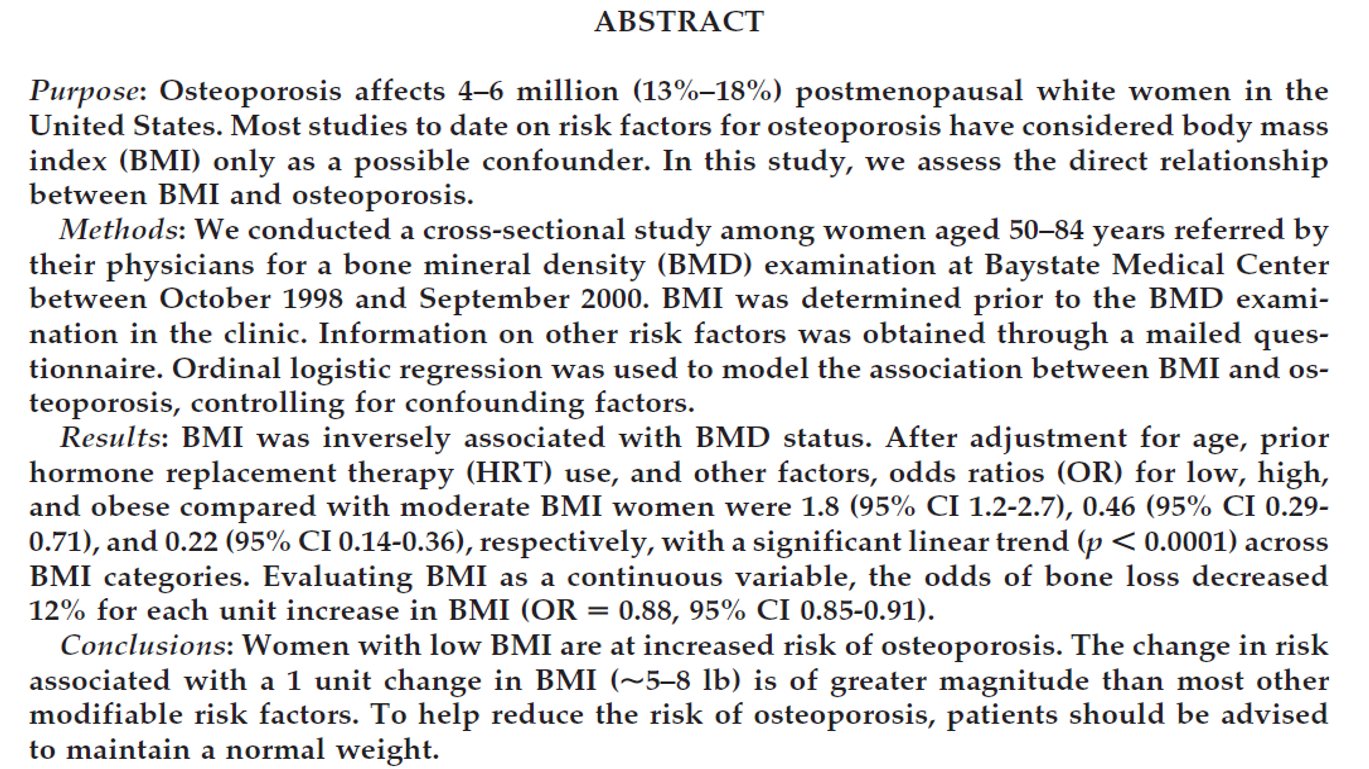
\includegraphics[width=1.175\textwidth]{Cap18-19/bmi-bmd-abstract}
  \end{center}
\end{frame}

\begin{frame}{Na prática...}
  \begin{columns}
    \begin{column}{5cm}
      \begin{itemize}
      \item Dados simulados, inspirados no paper.
      \item Existe uma tendência? Ela é linear?
      \item Podemos predizer a osteoporose a partir do IMC?
      \end{itemize}
    \end{column}
    \begin{column}{5cm}
      \begin{center}
        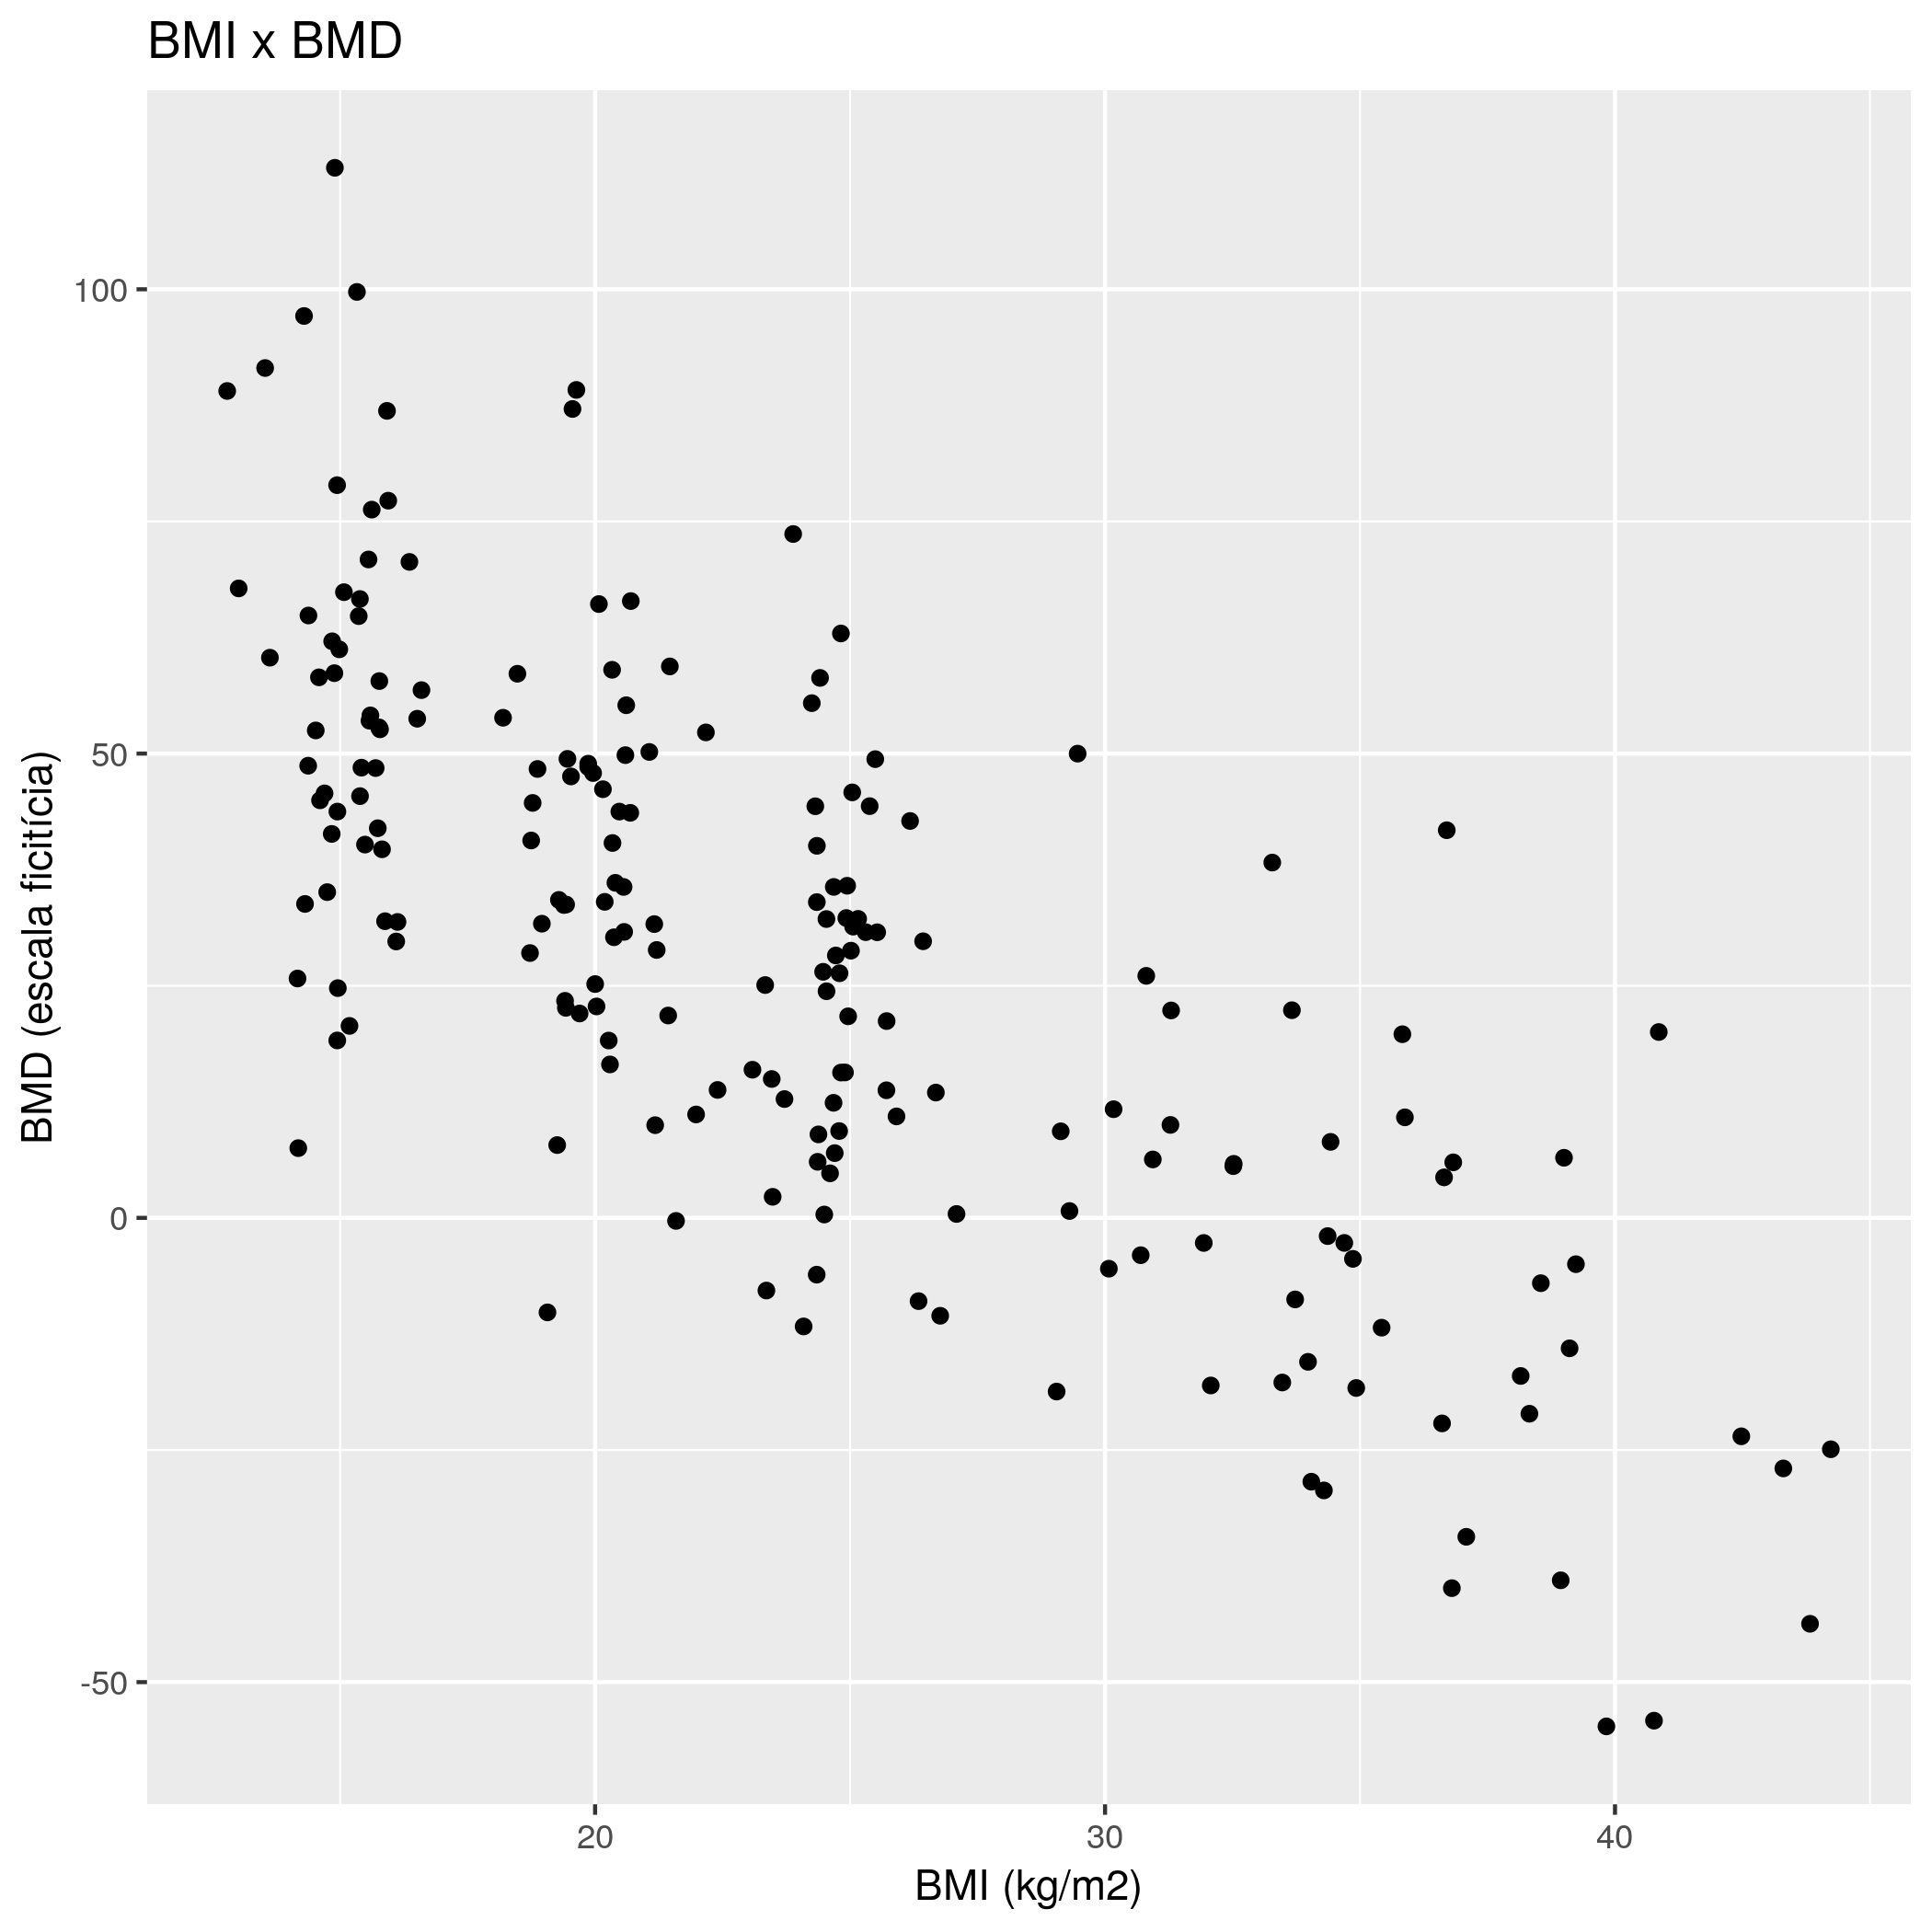
\includegraphics[width=\textwidth]{Cap18-19/pratica-plot1}
      \end{center}
    \end{column}
  \end{columns}
\end{frame}

\begin{frame}{Reta de regressão}
  \begin{definition}
    Uma \alert{reta de regressão} (também chamada de reta de melhor
    ajuste) é a reta para a qual a soma dos erros quadráticos dos
    resíduos é o mínimo.
  \end{definition}
  \begin{itemize}
  \item É a reta que melhor se ajusta aos dados
  \item Minimiza os resíduos
  \end{itemize}
\end{frame}

\begin{frame}{Resíduos}
  \begin{center}
      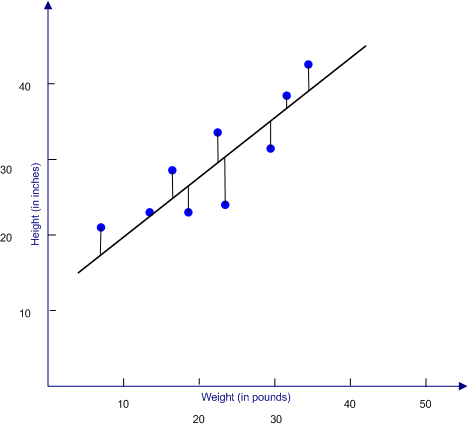
\includegraphics[height=0.6\textheight]{Cap18-19/residuos}
  \end{center}

  \begin{definition}
    Resíduos são a distância entre o dado observado e a reta estimada
    (modelo).
  \end{definition}
\end{frame}

\begin{frame}{Atenção}
  \begin{itemize}
  \item Para muitos testes presume-se que os dados vem de uma distribuição normal
  \item Neste caso, não é necessário que os {\bf dados} sejam normais
  \item {\bf É necessário que os resíduos sejam normais}
  \end{itemize}
\end{frame}

\begin{frame}{Elementos da reta de regressão}
  \begin{itemize}
  \item Relembrando: a equação de uma reta é definida pela fórmula
    \begin{displaymath}
      \hat{y} = \alert{a} x + \alert{b}
    \end{displaymath}
  \item No caso da reta regressora:
    \begin{itemize}
    \item $y$ é a variável dependente
    \item $x$ é a variável independente
    \item $a$ é a inclinação
    \item $b$ é o intercepto
    \end{itemize}
  \item Assim, o objetivo da análise de regressão é encontrar os
    valores \alert{$a$} e \alert{$b$}
  \end{itemize}
\end{frame}

\begin{frame}{Análise de Regressão}
  Para determinar a inclinação e o intercepto, usamos:
  \begin{itemize}
  \item as médias de $X$ e $Y$
  \item as variâncias de $X$ e $Y$
  \item o coeficiente de correlação $r$ entre $X$ e $Y$
  \item o tamanho da amostra $n$
  \item \ldots e algumas operações entre estes termos
  \end{itemize}
\end{frame}

\subsection{A regressão}

\begin{frame}{Exemplo}
  \begin{example}
    Voltemos ao exemplo de associar a composição lipídica com a sensibilidade a insulina.    
  \end{example}
  \begin{block}{Pergunta}
    Qual é o acréscimo na sensibilidade à insulina, para cada unidade aumentada na composição lipídica?
  \end{block}
\end{frame}

\begin{frame}{Exemplo}
  \centering
  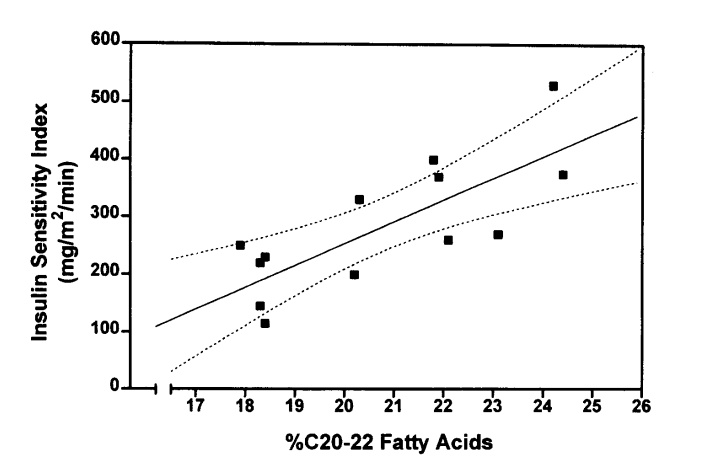
\includegraphics[width=.9\textwidth]{Cap18-19/regressao1}

  \vfill
  Fonte: Motulsky, 1995
\end{frame}

\begin{frame}{Exemplo}
  \centering
  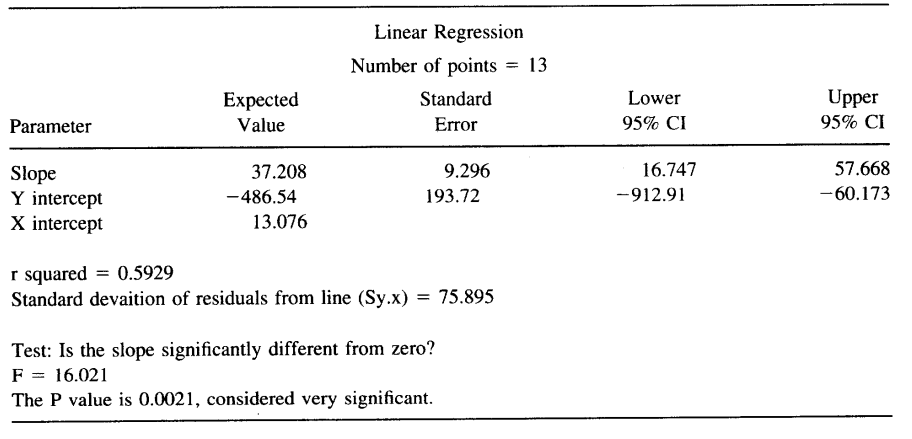
\includegraphics[width=1.2\textwidth]{Cap18-19/regressao2}
\end{frame}

\begin{frame}{Interpretação}
  \begin{itemize}
  \item O p-valor é significativo.
  \item A inclinação é $\approx \alert{37.2}$
  \item Isto significa que:
  \end{itemize}
  \begin{block}{}
    para cada unidade aumentada no \%C20--22, teremos um aumento proporcional de aproximadamente 37.2 mg/m$^2$/min na sensibilidade à insulina
  \end{block}
\end{frame}

\begin{frame}{Análise de Regressão}
  \begin{center}
      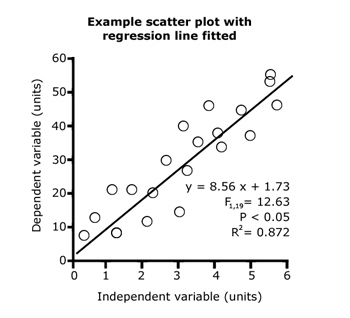
\includegraphics[height=0.6\textheight]{Cap18-19/residuos2}
  \end{center}

  \begin{itemize}
  \item A qualidade do ajuste do modelo de regressão é determinado
    pelo \alert{coeficiente de determinação} $r^2$
  % \item A semelhança de nomenclatura com o coeficiente $r$ não é mera
  %   coincidência.
  \end{itemize}
\end{frame}

  % Encontrando a inclinação e o intercepto da reta, podemos estimar
  % $\hat{Y}$ para valores arbitrários de $X$.

\subsection[$R^2$]{Coeficiente de Determinação $r^2$}

\begin{frame}{Coeficiente de Determinação $r^2$}
  \begin{definition}
    O \alert{coeficiente de determinação} $r^2$ é a relação da
    variação explicada com a variação total.
  \end{definition}
  \begin{displaymath}
    r^2 = \frac{\text{variação explicada}}{\text{variação total}}
  \end{displaymath}
  \begin{itemize}
  \item Lembrando: $r^2$ é o quadrado de $r$!
  % \item Este valor tem uma interpretação prática mais fácil, que
  %   veremos em breve
  \end{itemize}
\end{frame}

\begin{frame}{Coeficiente de Determinação $r^2$}
  \begin{itemize}
  % \item A variância dos dados pode ser explicada de várias formas
  \item Qual é a porcentagem da variação dos dados pode ser explicada
    pela reta regressora?
  \item O coeficiente $r^2$ é a fração da variância que é
    compartilhada entre $X$ e $Y$.
  \item Como $r$ está sempre entre -1 e 1, $r^2$ está sempre entre 0 e
    1.
  \end{itemize}
\end{frame}

\begin{frame}{Coeficiente de Determinação $r^2$}
  \begin{itemize}
  \item Além disso, $r^2 \le |r|$
  \item Por que?
  \end{itemize}
  \begin{block}{}
    Compare os seguintes números entre 0 e 1:
    \begin{displaymath}
      \frac{1}{2} \text{ e } \left(\frac{1}{2}\right)^2=\frac{1}{4} \Rightarrow
      \frac{1}{4} \le \frac{1}{2}
    \end{displaymath}
    \begin{displaymath}
      \frac{1}{3} \text{ e } \left(\frac{1}{3}\right)^2=\frac{1}{9} \Rightarrow
      \frac{1}{9} \le \frac{1}{3}
    \end{displaymath}
  \end{block}
\end{frame}


% \begin{frame}{Coeficiente de Determinação $r^2$}
%   \begin{itemize}
%   \item 
%   \end{itemize}
% \end{frame}

\subsection{Exercício}

\begin{frame}{Na prática...}
  \begin{center}
    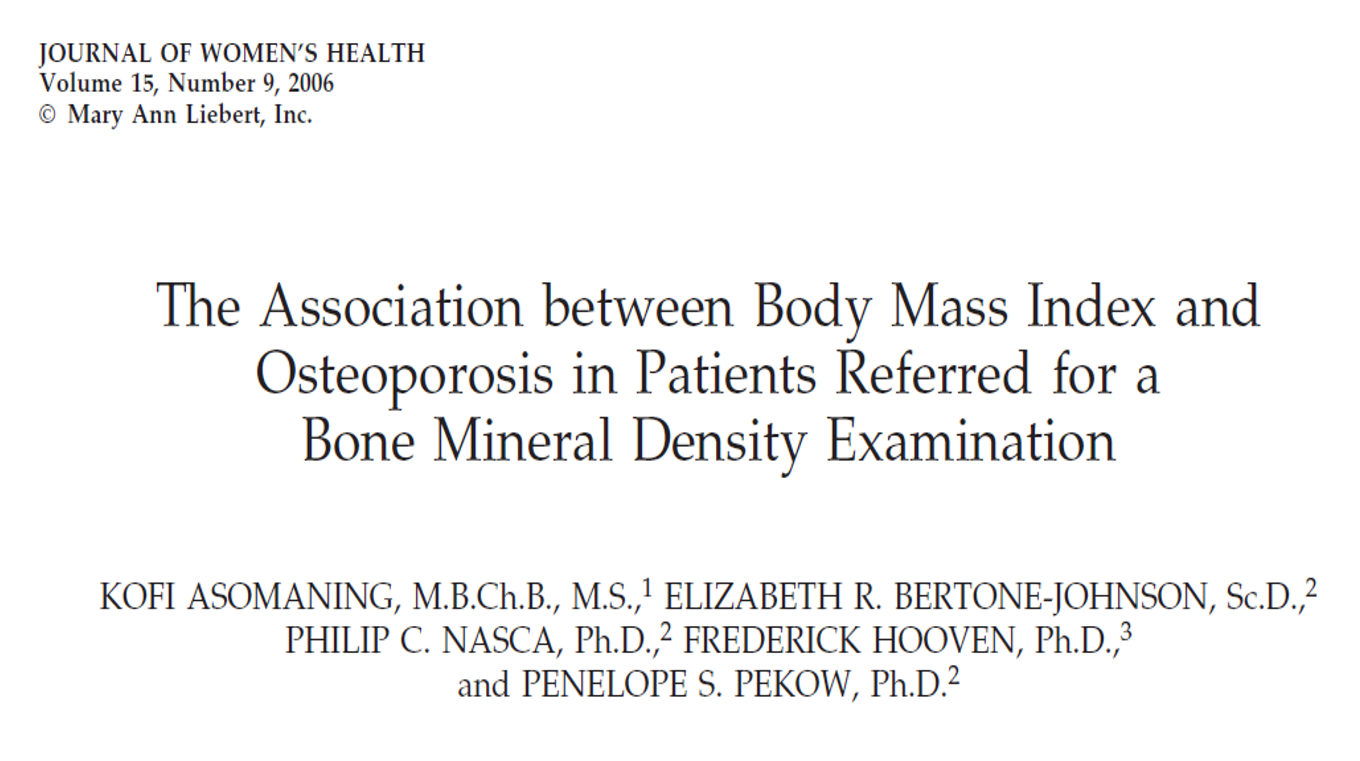
\includegraphics[width=\textwidth]{Cap18-19/bmi-bmd-title}
  \end{center}
\end{frame}

\begin{frame}{Na prática...}
  \begin{center}
    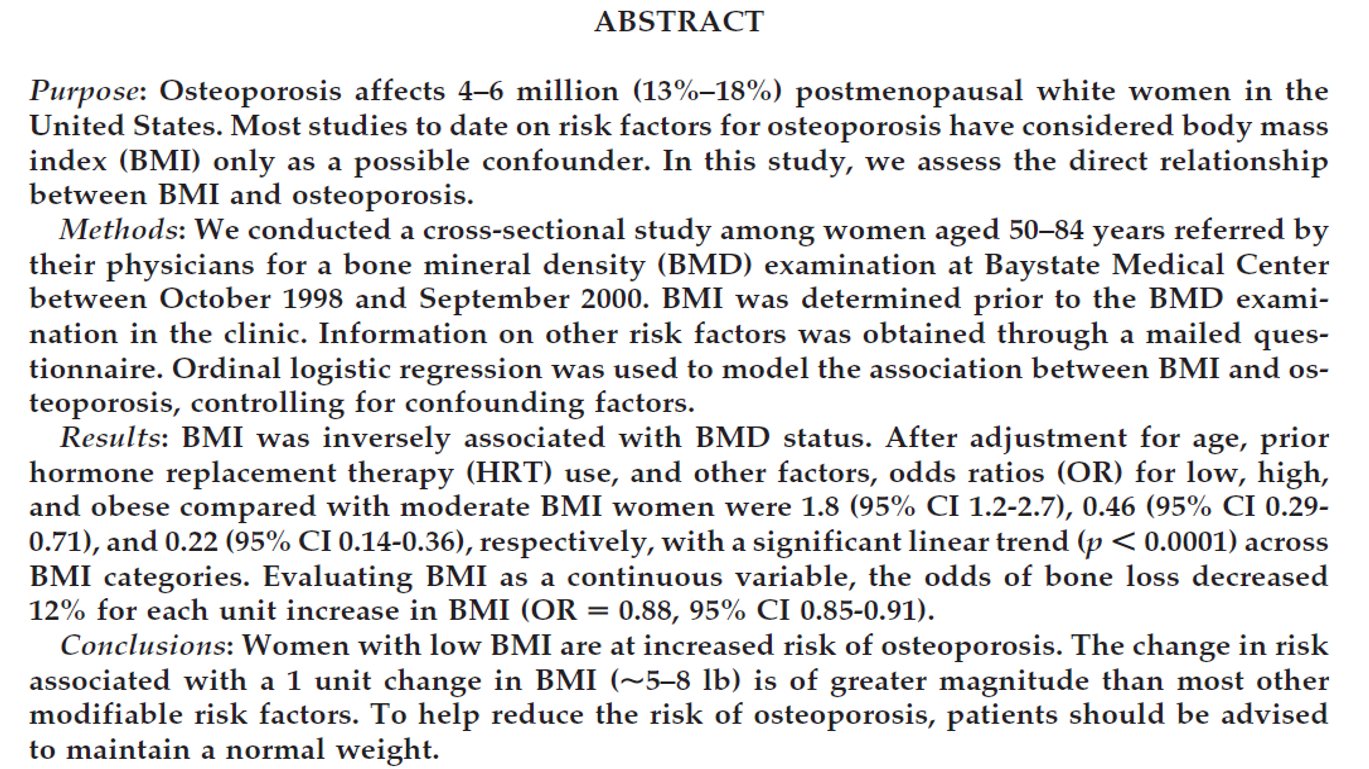
\includegraphics[width=1.175\textwidth]{Cap18-19/bmi-bmd-abstract}
  \end{center}
\end{frame}

\begin{frame}{Na prática...}
  \begin{center}
    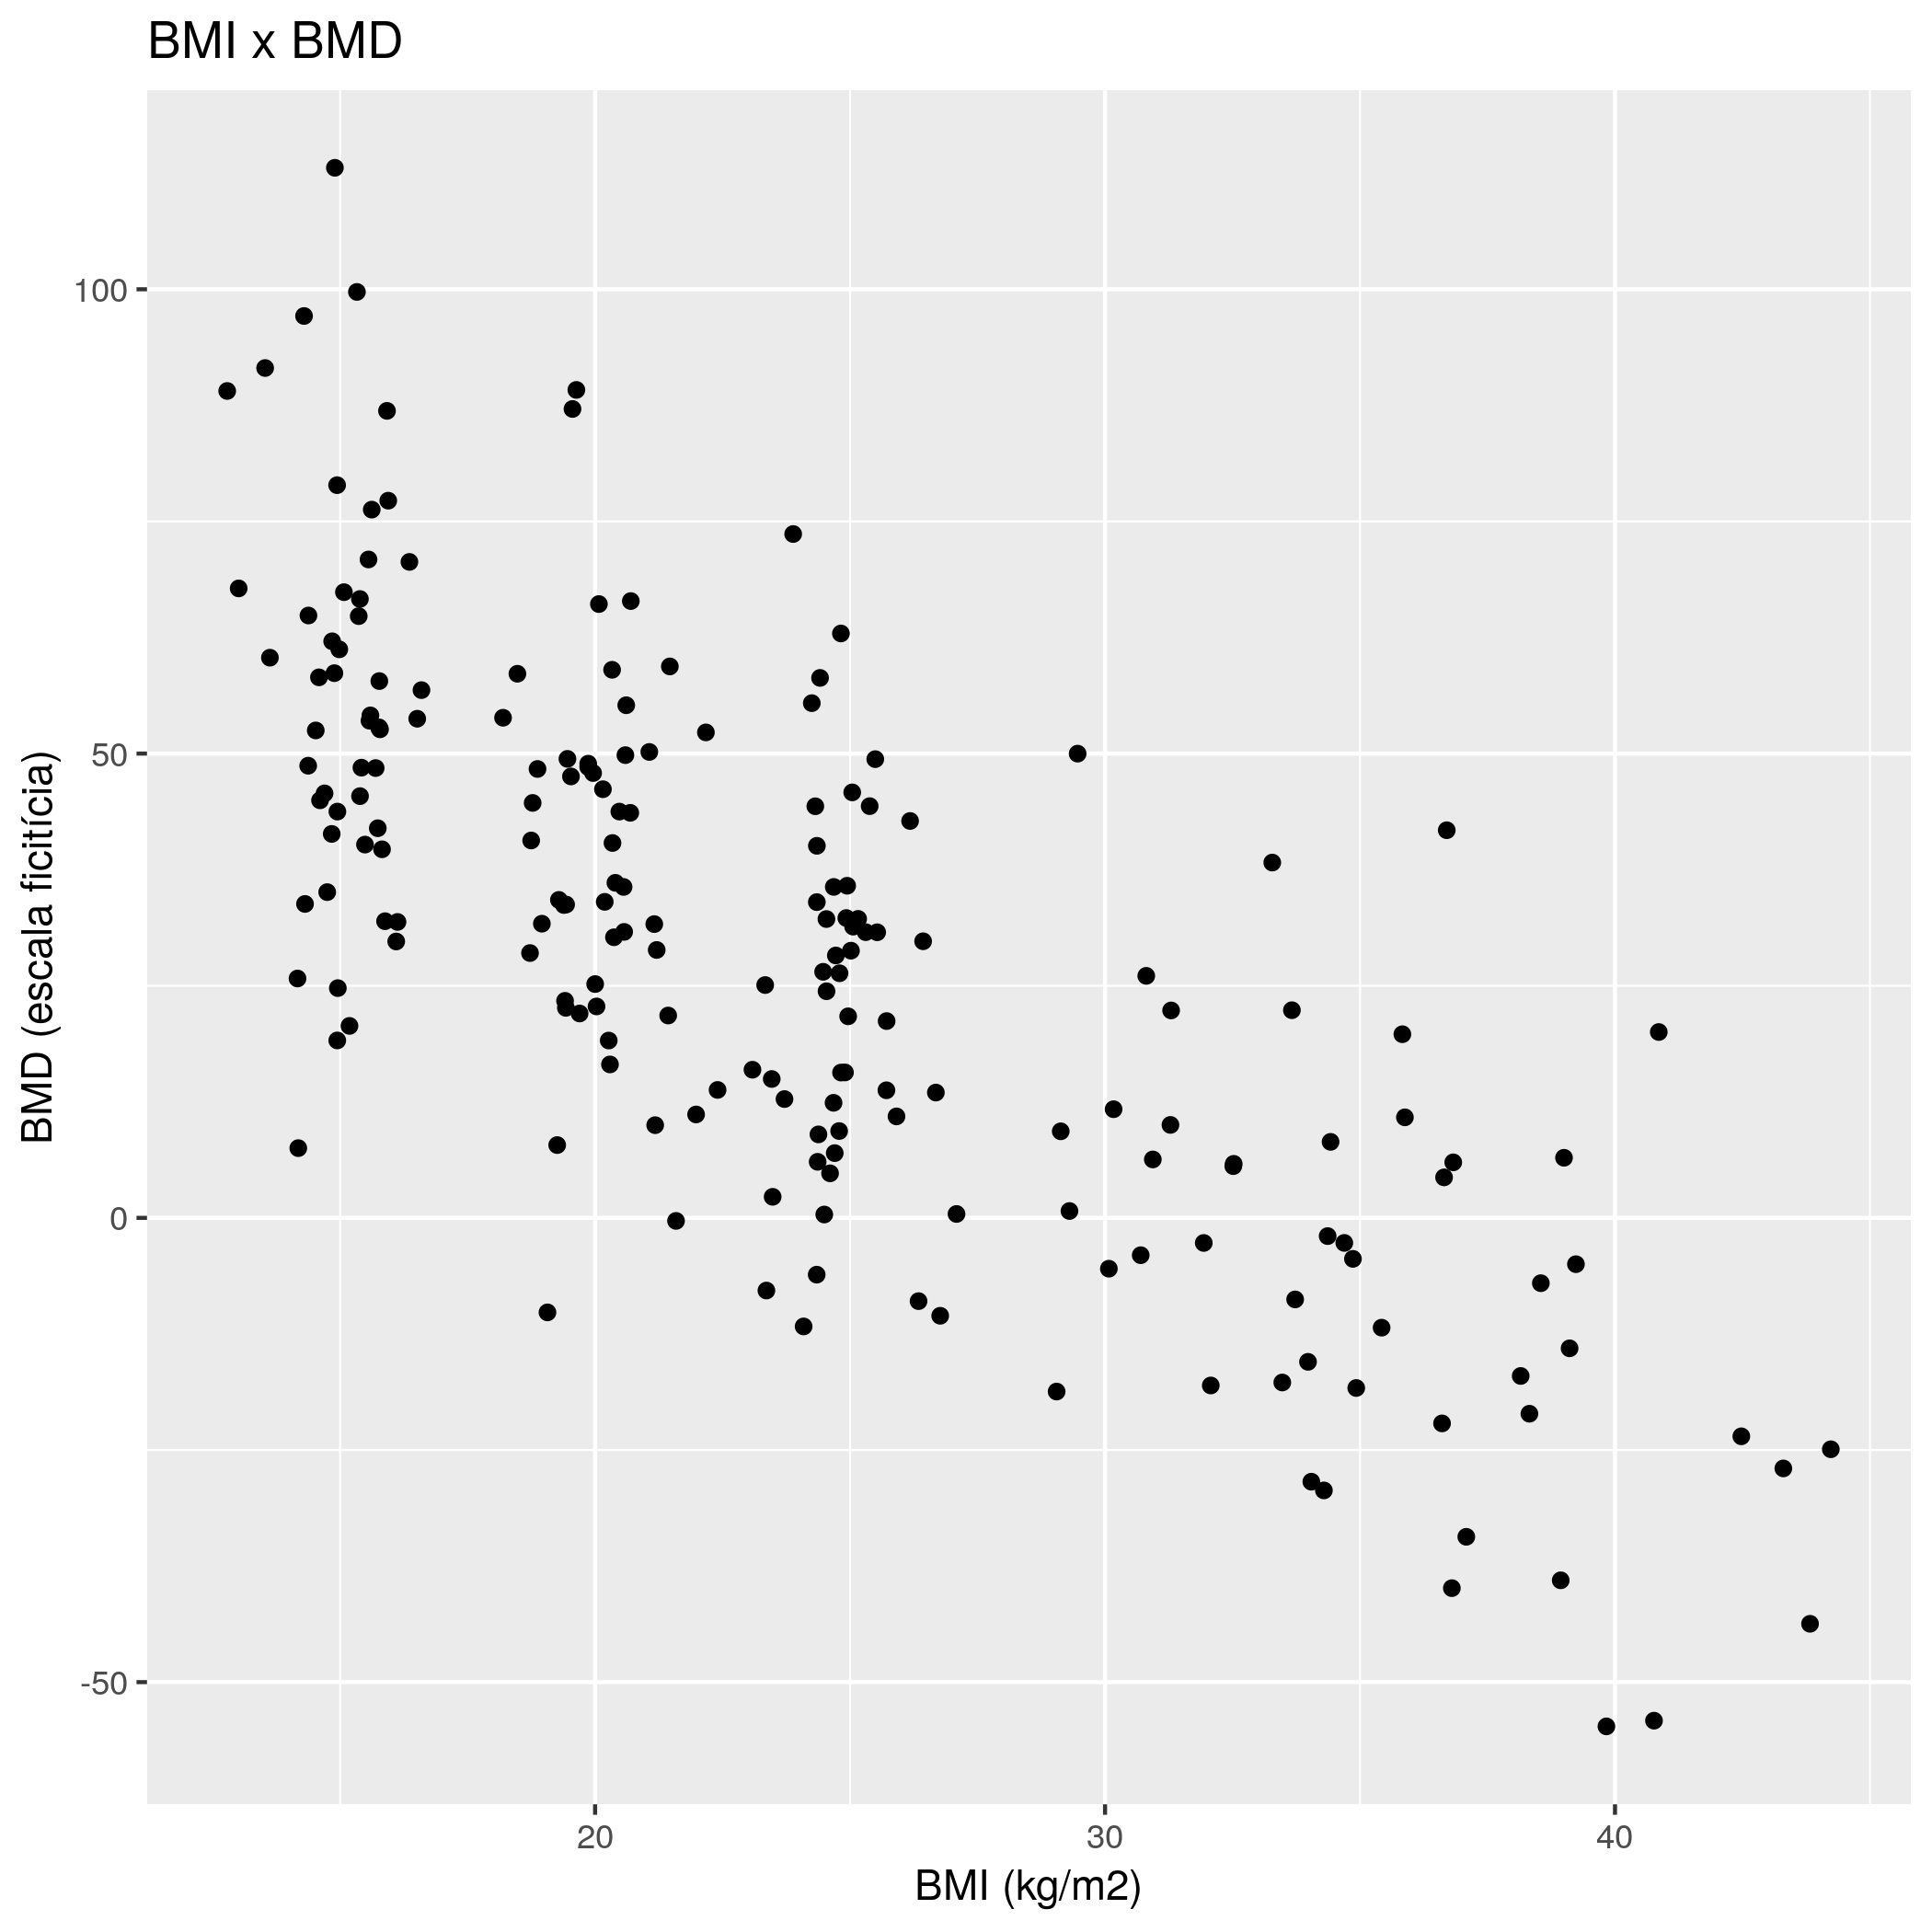
\includegraphics[height=.9\textheight]{Cap18-19/pratica-plot1}
  \end{center}
\end{frame}

\begin{frame}{Na prática...}
  \begin{center}
    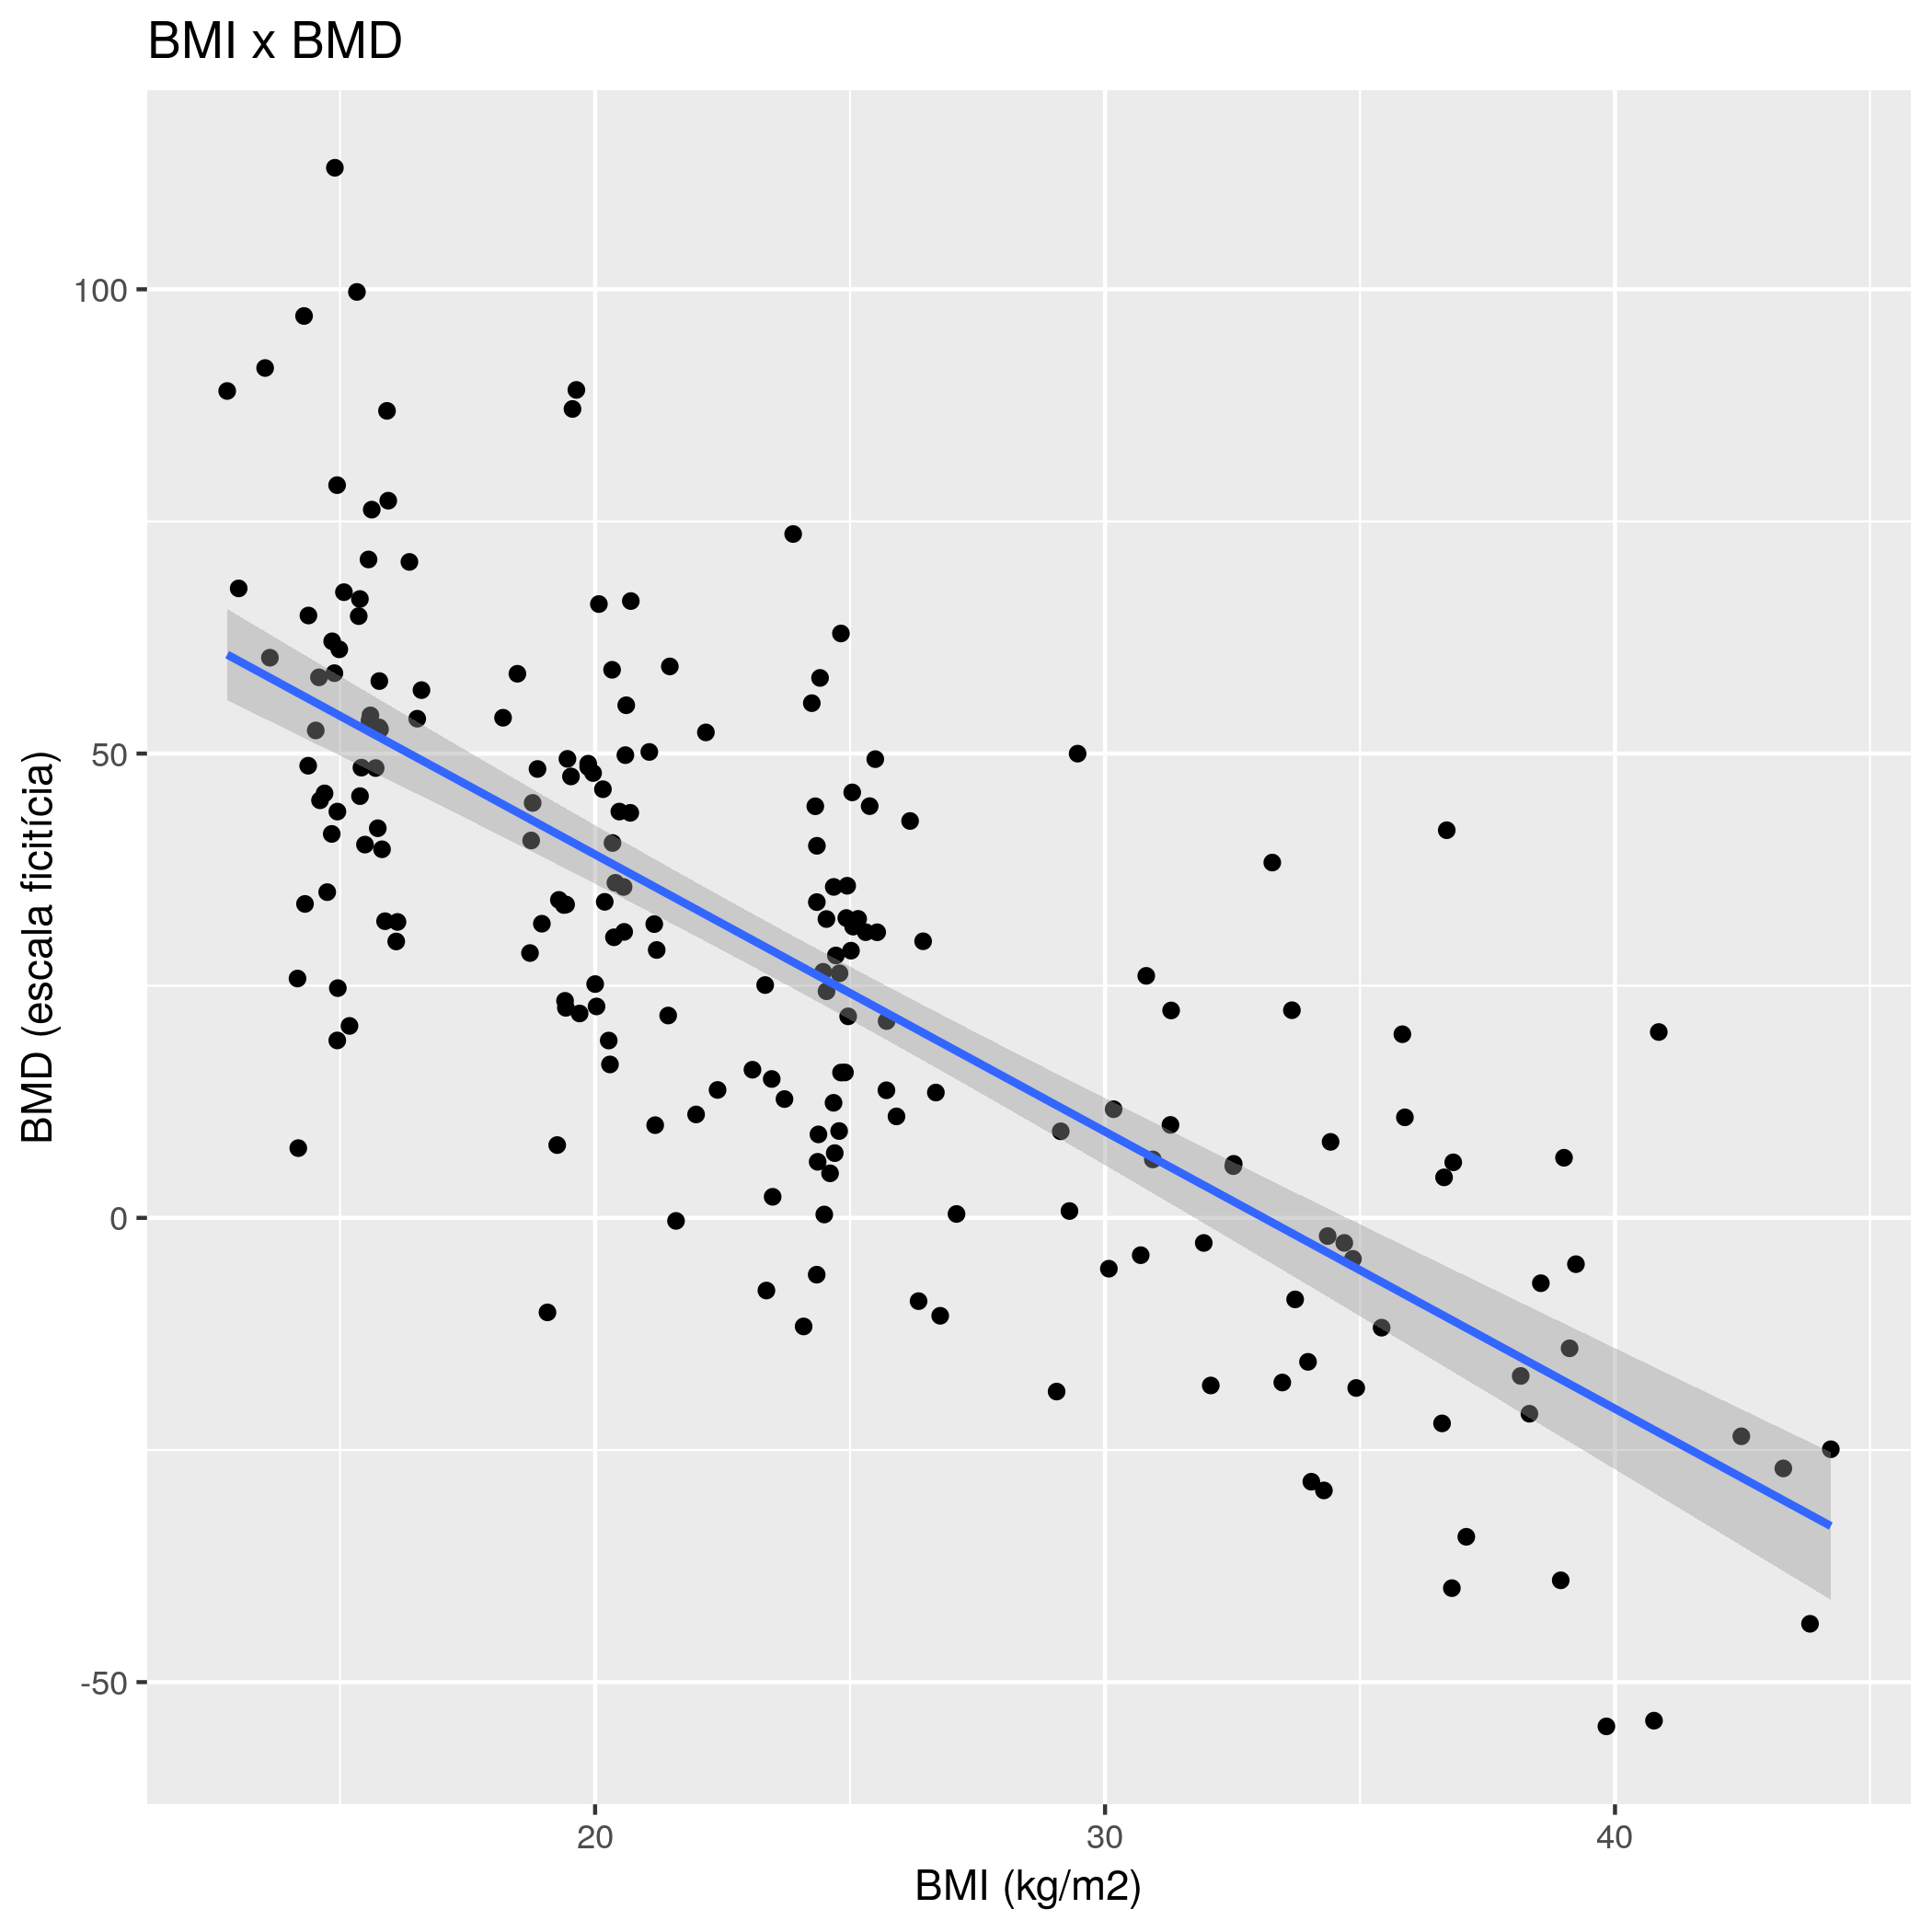
\includegraphics[height=.9\textheight]{Cap18-19/pratica-plot2}
  \end{center}
\end{frame}

\begin{frame}[fragile]{}
  \begin{exampleblock}{}
    \begin{itemize}
    \item Os resíduos são aprox. normais?
    \item Quantos \% de variabilidade podem ser explicados pelo modelo?
    \item Quanto o BMD muda, para cada unidade de BMI?
    \end{itemize}
  \end{exampleblock}
  \begin{exampleblock}{Saída títpica de um programa de análise}
    \tiny
\begin{verbatim}
Residuals:
    Min      1Q  Median      3Q     Max 
-52.097 -13.864   0.762  10.707  58.730 

Coefficients:
            Estimate Std. Error t value Pr(>|t|)    
(Intercept)  98.8176     4.6281   21.35   <2e-16 ***
BMI          -2.9845     0.1846  -16.17   <2e-16 ***
---
Signif. codes:  0 ‘***’ 0.001 ‘**’ 0.01 ‘*’ 0.05 ‘.’ 0.1 ‘ ’ 1

Residual standard error: 20.26 on 198 degrees of freedom
Multiple R-squared:  0.5691,	Adjusted R-squared:  0.5669 
F-statistic: 261.5 on 1 and 198 DF,  p-value: < 2.2e-16
\end{verbatim}
\end{exampleblock}
\end{frame}

\begin{frame}{E o BMI = 28?}
  \begin{center}
    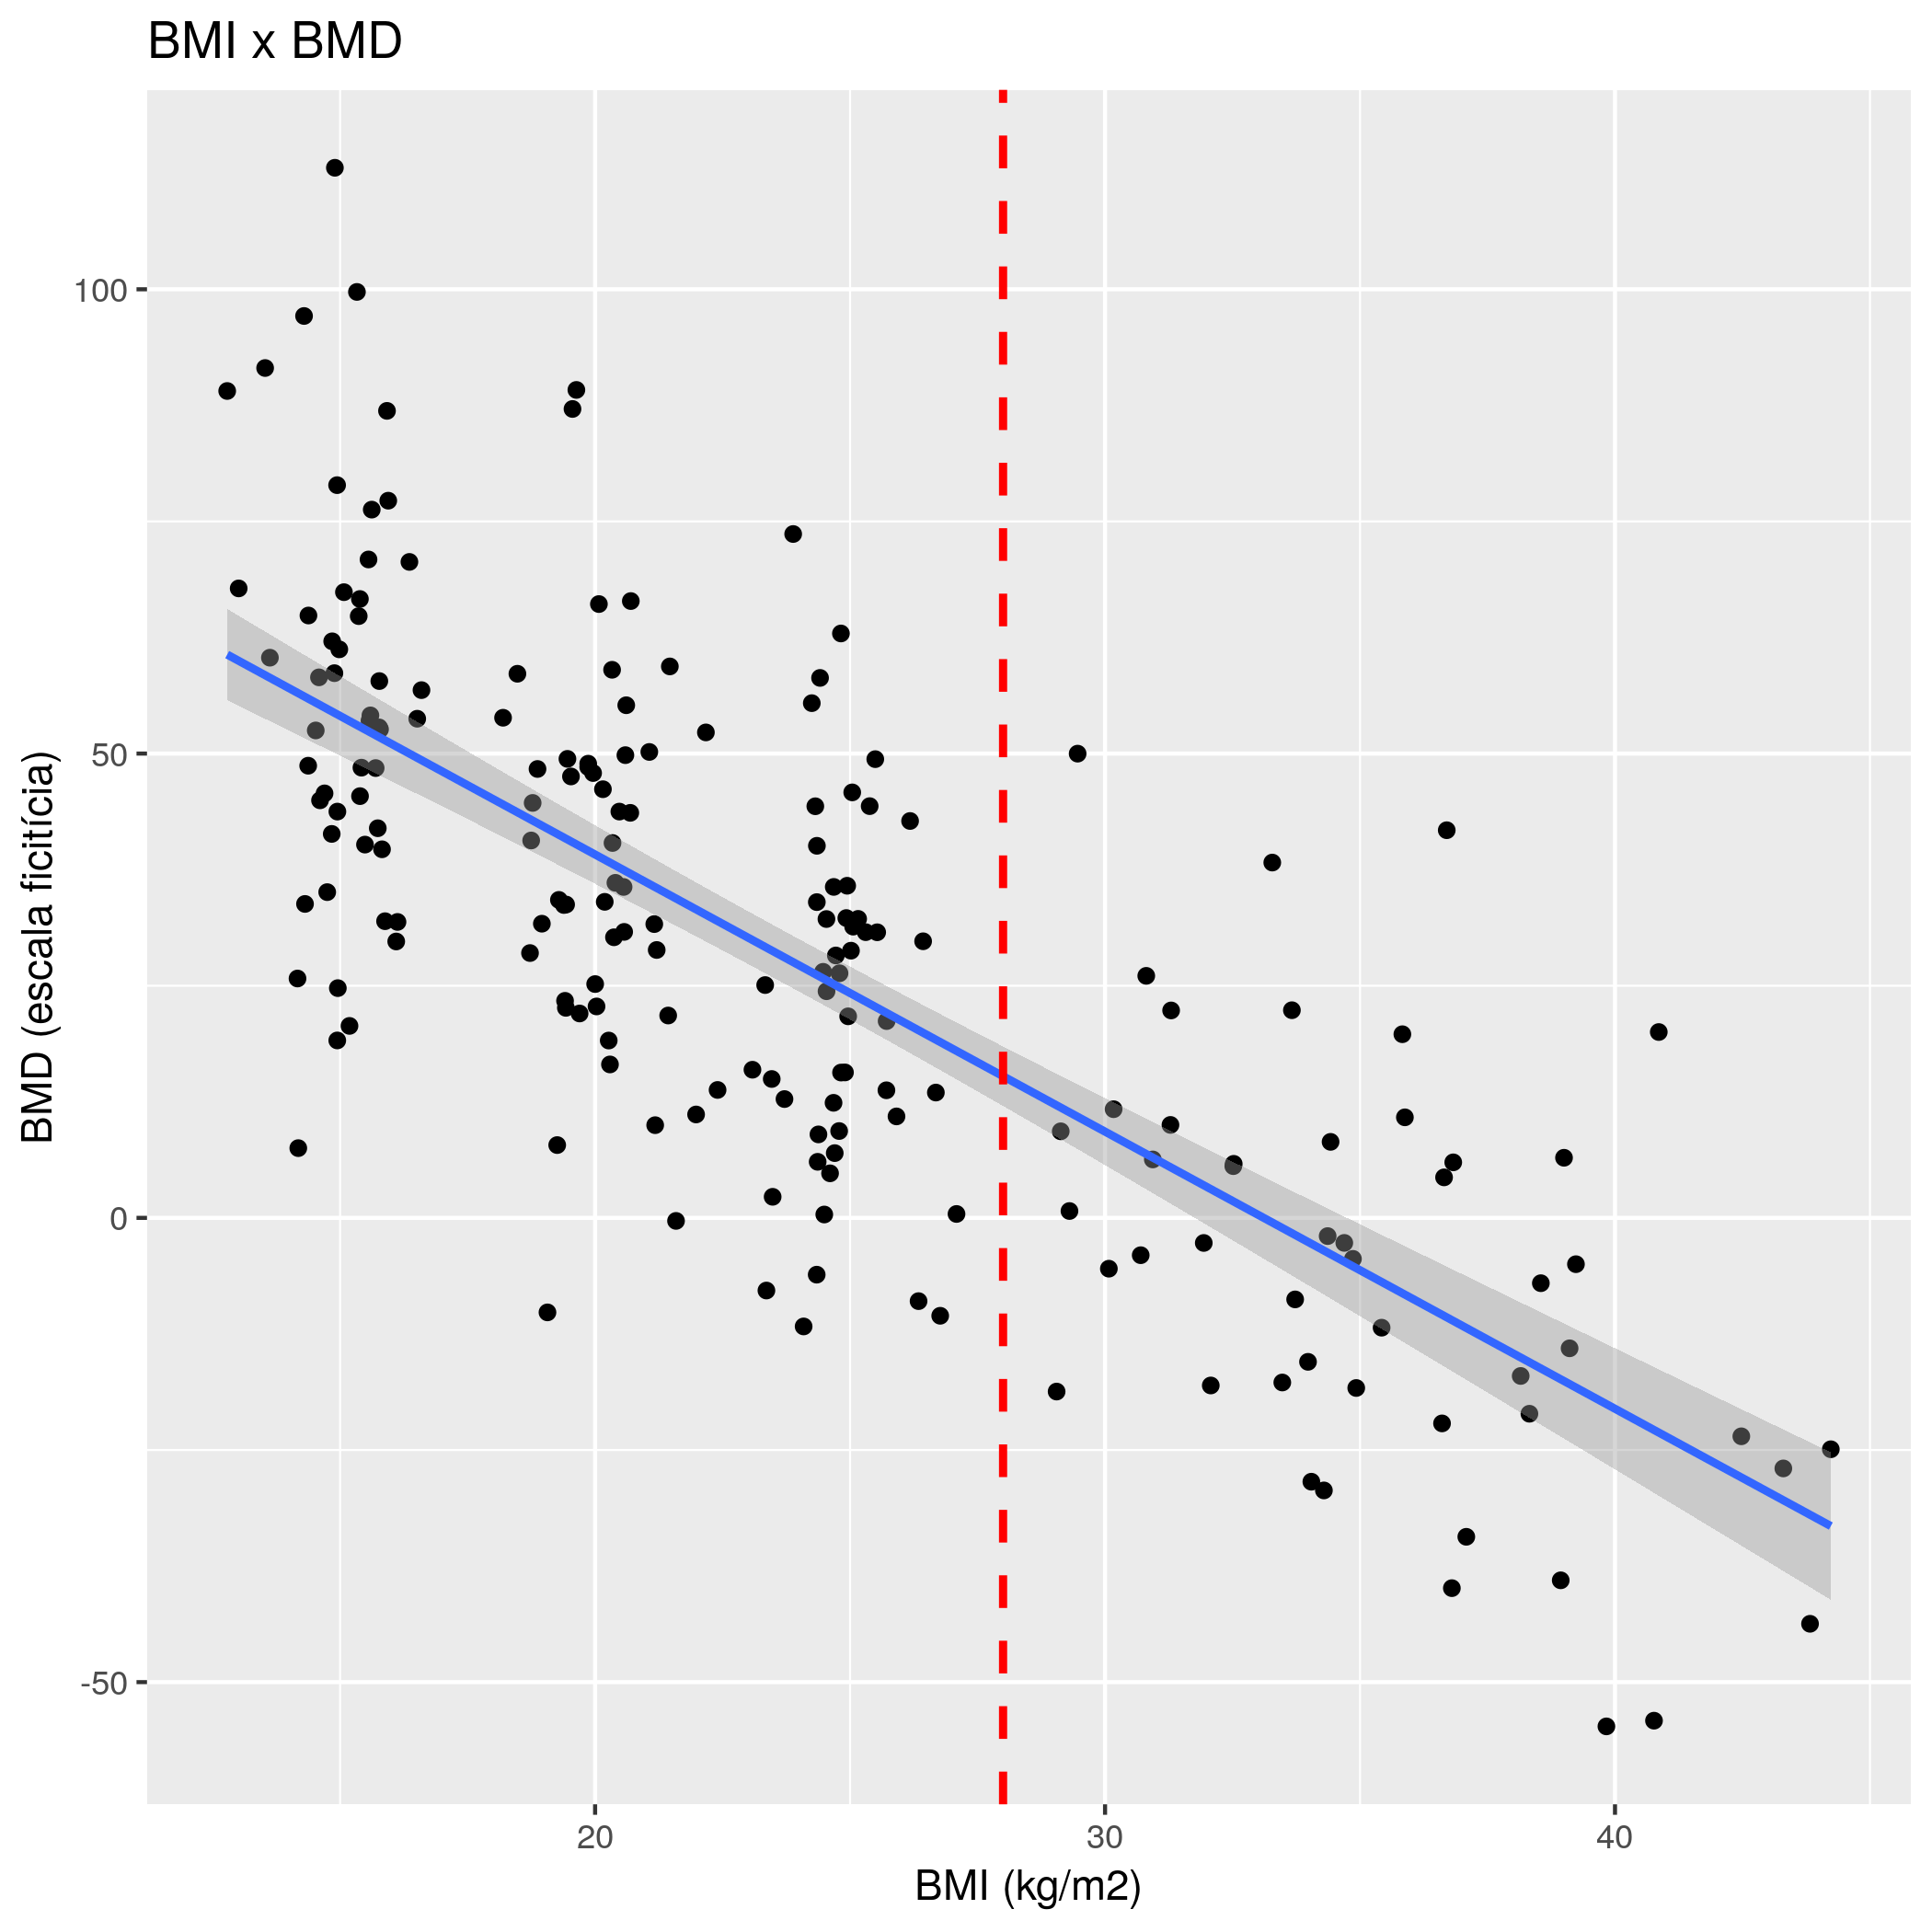
\includegraphics[height=.9\textheight]{Cap18-19/pratica-plot3}
  \end{center}
\end{frame}

\begin{frame}{E o BMI = 28?}
  \begin{itemize}
  \item o valor predito pelo modelo é 15.25169
  \item P: O que isto significa?
  \end{itemize}
\end{frame}

\section{Resumo}

\subsection{Resumo}

\begin{frame}{Resumo}
  \begin{itemize}
  \item É necessário investigar a relação entre as variáveis!
  \item O que pode explicar a relação observada?
  \item Qual proporção (porcentagem) da variabilidade pode ser
    explicada pelas variáveis analisadas?
  \item Quão bem a reta regressora se ajusta aos dados?
  \end{itemize}
\end{frame}

\begin{frame}{Leitura pós-aula e exercícios selecionados}
  \begin{block}{Leitura obrigatória}
    \begin{itemize}
    \item Capítulo 18
    \item Capítulo 19, pular as seções:
      \begin{itemize}
      \item regressão linear como método de mínimos quadrados
      \item calculando a regressão linear
      \end{itemize}
    \end{itemize}
  \end{block}
  \begin{block}{Exercícios}
    Capítulo 19, problemas: todos menos o problema 5.
  \end{block}
  \begin{block}{Leitura recomendada}
    \small
    
    \begin{itemize}
    \item Schneider A, Hommel G, Blettner M, 2010.
      \url{https://www.ncbi.nlm.nih.gov/pmc/articles/PMC2992018/}
    \item (paper do exercício) Asomaning, et al., 2006.
      \url{https://www.ncbi.nlm.nih.gov/pubmed/17125421}
    \end{itemize}
  \end{block}
\end{frame}

\end{document}
